\chapter{Implementacija i korisničko sučelje}
		
		
		\section{Korištene tehnologije i alati}
			
			Komunikacija u timu realizirana je korištenjem aplikacija MS Teams\footnote{https://www.microsoft.com/en-us/microsoft-365/microsoft-teams/group-chat-software}, WhatsApp\footnote{https://www.whatsapp.com/?lang=en} i Discord\footnote{https://discord.com/}. Za izradu UML dijagrama korišteni su alati Astah Professional\footnote{astah.net/products/astah-professional/} i Draw.io\footnote{https://app.diagrams.net/}. Kao sustav za upravljanje izvornim kodom korišten je Git\footnote{https://git-scm.com/}, a udaljenom repozitoriju projekta se može pristupiti na web platformi GitLab\footnote{https://gitlab.com/}.
			
			Kao razvojno okruženje korišten je Microsoft Visual Studio Code\footnote{https://code.visualstudio.com/}, te Eclipse\footnote{https://www.eclipse.org/} i IntelliJ\footnote{https://www.jetbrains.com/idea/} za dijelove koda pisane u Javi. Visual Studio Code je besplatan editor izvornog koda razvijen od tvrtke Microsoft za Windows, Linux i macOS. Njegove značajke uključuju podršku za debuggiranje, isticanje sintakse, inteligentno završavanje napisanog koda, refakotoriranje koda i ugrađen Git. IntelliJ i Eclipse su IDEvi razvijeni za programski jezik Java.
			
			Aplikacija je napisana koristeći Express\footnote{https://expressjs.com/} radni okvir i jezik Javascript za izradu backenda te Node.js\footnote{https://nodejs.org/en/} i pug\footnote{https://pugjs.org/api/getting-started.html} za izdradu frontenda. Node.js je kao asikroni i događajima-pokrenut JavaScript runtime dizajniran za izradu skalabilnih web aplikacija. Pug je HTML-ov predprocesor.
			
			Za prikaz karte i lokacije parkinga korišten je Google Maps api\footnote{https://developers.google.com/maps/documentation/javascript/overview}. Za potrebe baze podataka korišten je PostgreSQL\footnote{https://www.postgresql.org/}. Sama aplikacija i baza podataka je objavljena na cloud platformi Heroku\footnote{https://www.heroku.com/}.
			
			Za potrebe sistemskog testiranja aplikacije korišten je Selenium\footnote{https://www.selenium.dev/} i jezik Python (koristeno razvojno okruzenje Pycharm\footnote{https://www.jetbrains.com/pycharm/}). Selenium je prijenosni radni okvir za testiranje web aplikacija. Pruža alat za pravljenje funkcionalnih testova bez potrebe da se uči skriptni jezik za testiranje.\newline
			Za testiranje Node.js funkcija korišten je Mocha\footnote{https://mochajs.org/}. Kao napredni uređivač teksta korišten je Sublime\footnote{https://www.sublimetext.com/}.
			
			
			\eject 
		
	
		\section{Ispitivanje programskog rješenja}
							
			Ispitivanje (testiranje) se provelo u dva oblika. Prvi je kroz sistemske, a drugi kroz \textit{unit} testove. 
			Sistemskim testovima testiran je dio sustava (aplikacije), a \textit{unit} testovima manji segment (funkcija) u kodu.
			
			Sistemskim testovima provjerena je funkcionalnost registracije korisnika, registracija tvrtke, prijava korisnika, prijava tvrtke, dodavanje automobila (korisnička funkcionalnost) te promjena imena (korisnička funkcionalnost).
			
		
			
			
			\subsection{Ispitivanje komponenti}
			
			Testiranje je obavljeno u Node.js-u pomoću Mocha-e.\newline
			
			Testiranjem komponenti željelo se provjeriti ispravnost funkcija napisanih na klijentskoj strani. Ovim testovima provjeravalo se dohvaćanje korisničkih podataka (ime i prezime), dohvaćanje lokacije (preko ID-a i koordinata), dohvaćanje rezervacija i dohvaćanje vozila.\newline
			
			U nastavku je prikazan kod i rezultati testiranja.
	
			%unos slike
			\begin{figure}[H]
				\begin{lstlisting}
					const assert = require('chai').assert;
					const KorisnikPodatci = require('../tools/KorisnikPodatci');
					
					describe('KorisnikPodatci', async function(){
						it('Trebao bi vratiti test', async function(){
							const vozac = await KorisnikPodatci.dohvatiVozacaPrekoUsernamea('testuser');
							assert.equal(vozac.imeVozac, 'test');
						});
						
						it('Trebao bi vratiti test', async function(){
							const vozac = await KorisnikPodatci.dohvatiVozacaPrekoUsernamea('testuser');
							assert.equal(vozac.prezimeVozac, 'test');
						});
					});
				\end{lstlisting}
				
				\centering
				\caption{Prikaz testa dohvaćanja korisničkih podataka}
				\label{fig:test - user - dohvacanje korisničkih podataka}
			\end{figure}
	

	


			%unos slike
			\begin{figure}[H]
				\begin{lstlisting}
					const assert = require('chai').assert;
					const LokacijaPodatci = require('../tools/LokacijaPodatci');
					const Lokacija = require('../models/Lokacija')
					
					describe('LokacijaPodatci', async function(){
						it('Trebao bi vratiti 36', async function(){
							lokacijaBezId = new Lokacija('trg bana josipa jelacica', 45.813264153294114, 15.977233094526218);
							const lokacija= await LokacijaPodatci.dohvatiIdLokacije(lokacijaBezId);
							assert.equal(lokacija[0].idlokacija, 36);
						});
					});
				\end{lstlisting}
			
				\centering
				\caption{Prikaz testa dohvaćanja lokacije preko id-a}
				\label{fig:test - user - dohvaćanje lokacije preko id-a}
			\end{figure}
				
			%unos slike
			\begin{figure}[H]
				
				\begin{lstlisting}
					const assert = require('chai').assert;
					const ParkingPodatci = require('../tools/ParkingPodatci');
					
					describe('LokacijaPodatci', async function(){
						it('Postoje dva parkinga sa istom lokacijom \
						(moze se dogodit da neka tvrtka slucajno doda),\
						pa se vraca samo jedna', async function(){
							//jelacic koordinate, ima dvije lokacije
							let parking = await ParkingPodatci.dohvatiParkingZaKoordinate(
							45.813264153294114, 15.977233094526218);
							assert.equal(parking.idlokacija, 35);
						});
					});
				\end{lstlisting}
				
				\centering
				\caption{Prikaz testa dohvaćanja lokacije preko koordinata}
				\label{fig:test - user - dohvaćanje lokacije preko koordinata}
			\end{figure}
				
			%unos slike
			\begin{figure}[H]
				
				\begin{lstlisting}
					const assert = require('chai').assert;
					const RezervacijaPodatci = require('../tools/RezervacijaPodatci');
					const KorisnikPodatci = require('../tools/KorisnikPodatci');
					
					
					describe('RezervacijaPodatci', async function(){
						it('Trebao bi vratiti sava, tvrtka, 500, test', async function(){
							vozac = await KorisnikPodatci.dohvatiVozacaPrekoUsernamea('testuser')
							rezervacije = await RezervacijaPodatci.dohvatiRezervacije(vozac);
							assert.equal(rezervacije[0].adresalokacija, 'sava');
							assert.equal(rezervacije[0].korisnickoimetvrtke, 'tvrtka');
							assert.equal(rezervacije[0].kapacitet, 500);
							assert.equal(rezervacije[0].registracija, 'test');
						});
					});
				\end{lstlisting}
			
				\centering
				\caption{Prikaz testa dohvaćanja rezervacija}
				\label{fig:test - user - dohvaćanje rezervacija}
			\end{figure}
				
			%unos slike
			\begin{figure}[H]
				\begin{lstlisting}
					const assert = require('chai').assert;
					const VoziloPodatci = require('../tools/VoziloPodatci');
					const KorisnikPodatci = require('../tools/KorisnikPodatci');
					const Vozilo = require('../models/Vozilo')
					const chai = require('chai')
					const expect = chai.expect
					chai.use(require('chai-as-promised'))
					
					describe('VoziloPodatci', async function(){
						it('Trebao bi vratiti test, auto1, auto2', async function(){
							vozac = await KorisnikPodatci.dohvatiVozacaPrekoUsernamea('testuser')
							const vozila = await VoziloPodatci.dohvatiVozila(vozac);
							assert.equal(vozila[0].registracija, 'test');
							assert.equal(vozila[1].registracija, 'auto1');
							assert.equal(vozila[2].registracija, 'auto2');
						});
						
						it('Trebao bi vratiti 4, 3, noviauto', async function(){
							vozac = await KorisnikPodatci.dohvatiVozacaPrekoUsernamea('testuser')
							vozilo = new Vozilo('noviauto', vozac);
							await VoziloPodatci.dodajVozilo(vozilo, vozac);
							let vozila = await VoziloPodatci.dohvatiVozila(vozac);
							assert.equal(vozila.length, 4);
							await VoziloPodatci.ukloniVozilo(vozac, 'noviauto');
							vozila = await VoziloPodatci.dohvatiVozila(vozac);
							assert.equal(vozila.length, 3);
						});
						
						it('Trebao bi biti error', async function(){
							vozac = await KorisnikPodatci.dohvatiVozacaPrekoUsernamea('testuser')
							vozilo = new Vozilo('   ', vozac);
							await expect(VoziloPodatci.dodajVozilo(vozilo, vozac)).to.be.rejectedWith(Error)
						});
						
					});
				\end{lstlisting}
				
			
				\centering
				\caption{Prikaz testa dohvaćanje vozila}
				\label{fig:test - user - dohvaćanje vozila}
			\end{figure}
				
			%unos slike
			\begin{figure}[H]
				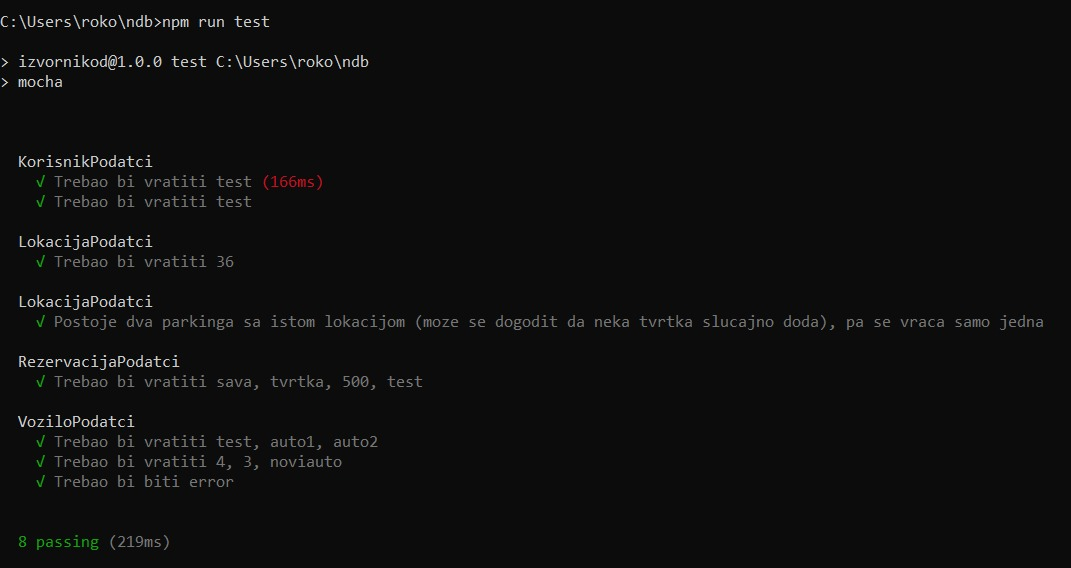
\includegraphics[scale=0.4]{slike/test_unit_testsOK.jpg} %veličina slike u odnosu na originalnu datoteku i pozicija slike
				\centering
				\caption{Prikaz prolaza svih testova}
				\label{fig:test - user - prolaz svih testova}
			\end{figure}
	
			%unos slike
			\begin{figure}[H]
				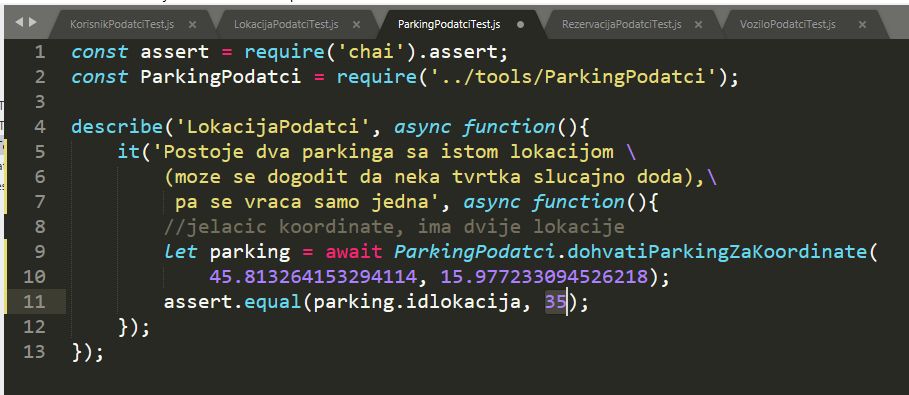
\includegraphics[scale=0.6]{slike/test_unit_kriviTest.png} %veličina slike u odnosu na originalnu datoteku i pozicija slike
				\centering
				\caption{Prikaz testa u kojem se očekuje drugačija vrijednost od dobivene (označena razlika u odnosu na prijašnji test)}
				\label{fig:test - user - test s neocekivanom vrijednosti}
			\end{figure}		
		
		
			%unos slike
			\begin{figure}[H]
				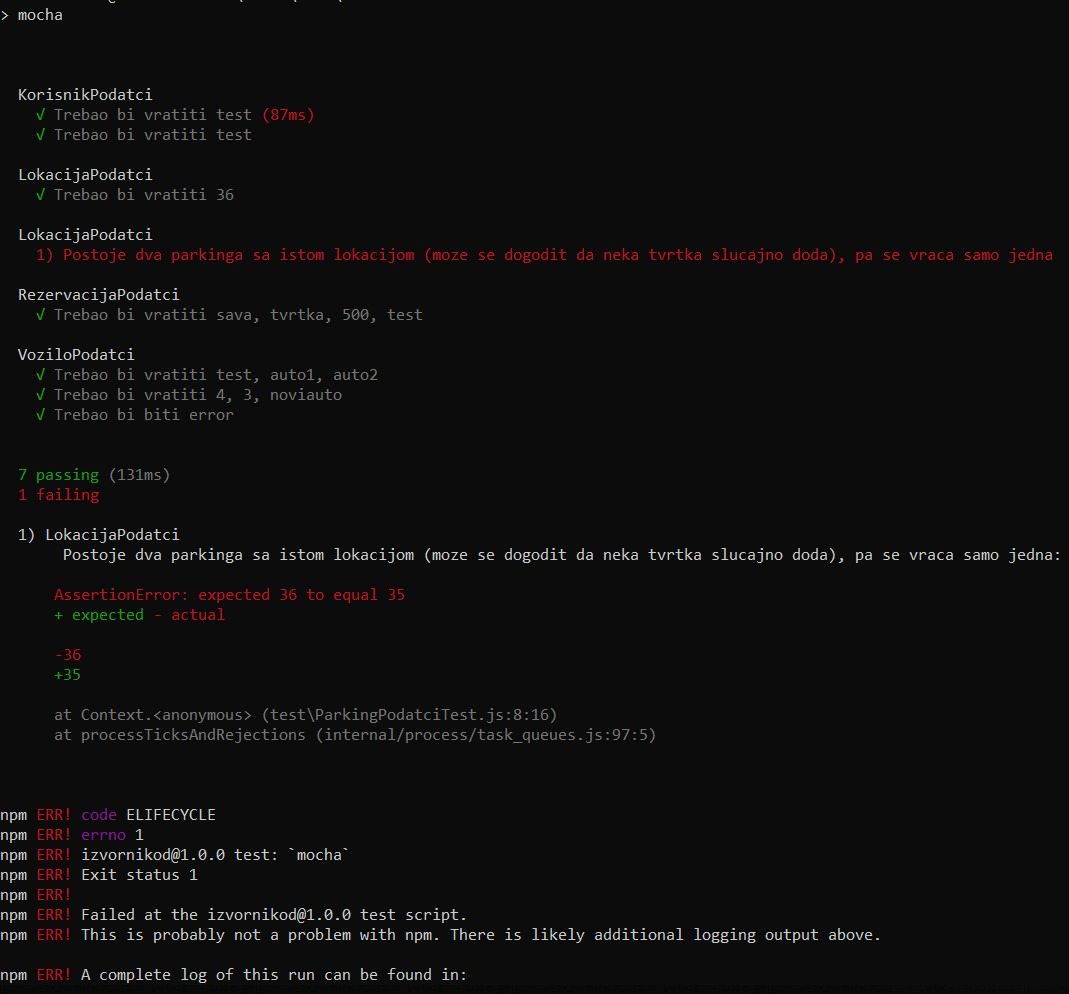
\includegraphics[scale=0.4]{slike/test_unit_testNeOK.jpg} %veličina slike u odnosu na originalnu datoteku i pozicija slike
				\centering
				\caption{Prikaz neprolaženja svih testova}
				\label{fig:test - user - neprolazenje svih testova}
			\end{figure}	
				
			\subsection{Ispitivanje sustava}
							
					Kod za testiranje je pisan u Pythonu, Selenium je korišten za interakciju s elementima u aplikaciji.
			
			Kao pripremu za testiranje registracija napravljene su baze podataka koje sadrže nasumično generirane parametre (ime, prezime, broj kartice i slično). Prilikom registracije dohvaća se jedan set podataka koji se koriste za registraciju te se nakon toga bilježi kako su ti podatci iskorišteni, pri idućoj registraciji dohvaća se novi set podataka. Proces je iterativan. 
			Razlog ovakvog pristupa naspram ustaljenog (procedure koja prije pokretanja testa registracije briše testnog korisnika ili tvrtku kako bi se mogao ponovno koristiti taj isti korisnik ili tvrtka za registraciju) je što se ovako ostvaruje dualna funkcija; \underline{testiranje} i \underline{pisanje} podataka u bazu. Drugo ima za posljedicu lakše ručno testiranje svih funkcionalnosti vezanih uz korisnike i tvrtke pošto su već upisani u bazi te se ne treba stvarati ispitni skup korisnika i tvrki (na primjer: kako bi se testirale administratorske ovlasti nad njima)
			
			Druga priprema koja je napravljena na \textit{home} stranici je pridruživanje svakom relevantnom elementu za testiranje \textit{id}. Svaki \textit{id} je broj, te su vrijednosti posložene tako da se pri testiranju može iterirati po određenom spektru tih brojeva i jednostavno dohvaćati elemente, pritiskati na njih i upisivati u njih željene znakove. 
					
			
			%unos slike
			\begin{figure}[H]
				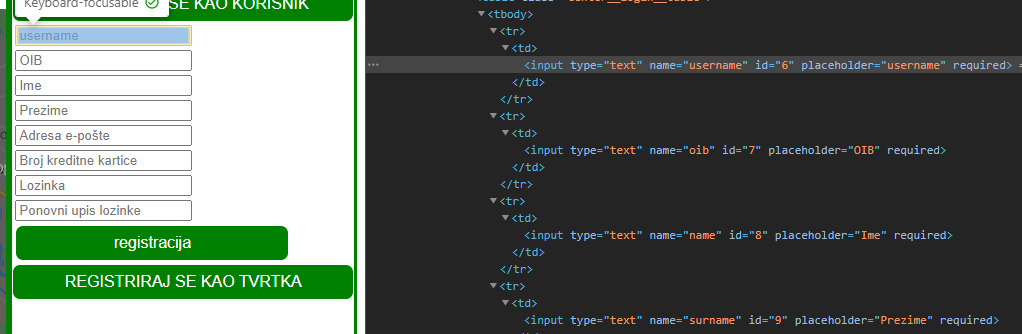
\includegraphics[scale=0.6]{slike/html_id.png} %veličina slike u odnosu na originalnu datoteku i pozicija slike
				\centering
				\caption{Prikaz enumeracije \textit{id}-eva}
				\label{fig:promjene}
			\end{figure}
		
			U nastavku je prikaz koda i rezultata testiranja.
			Većina testova koristi \textit{driver} koji obavlja test s predanim parametrima koje mu određeni test predaje.
			Svi testovi se nalaze u klasi \textit{TestApp}.
			
			%unos slike
			\begin{figure}[H]
				\begin{lstlisting}
				# ... importi
				
				class TestApp(unittest.TestCase):
				
					PAGE_URL = "http://127.0.0.1:3000/"
					SHOW_LOG = False
					USER_USERNAME = "marin"
					USER_PASSWORD = "123123"
					
					IS_ALL_OK = True
					
					driver = webdriver.Chrome(ChromeDriverManager().install())
					
				# ... nastavak koda
				\end{lstlisting}
		
				\centering
				\caption{Prikaz varijabli i konstanti}
				\label{fig:test - sistemski- varijable i konstante}
			\end{figure}
		
					
			%unos slike
			\begin{figure}[H]
				
				\begin{lstlisting}
					# ... unutar TestApp
					
					def login_driver(self, username, password, invert_score=False):
						driver = self.driver
						
						try:
							driver.get(self.PAGE_URL)
							time.sleep(4)
							
							i_0 = 2
							credentials = [username, password]
							
							for i_1 in credentials:
								user = driver.find_element_by_id(i_0)
								user.click()
								user.send_keys(i_1)
								i_0 += 1
							
							user = driver.find_element_by_id(i_0)
							user.click()
							
							time.sleep(4)
							try:
								tester = driver.find_element_by_id("name_ph")
							except:
								raise self.FailTest("login nije uspjesno napravljen")
								
							self.assertTrue(not invert_score)
							
						except self.FailTest as e:
							self.IS_ALL_OK = False
							print(e)
							
							self.assertTrue(invert_score)
							
						except:
							self.IS_ALL_OK = False
							import sys
							print(sys.exc_info()[0])
							self.assertTrue(False)
				\end{lstlisting}
				
				\centering
				\caption{Prikaz login drivera}
				\label{fig:test - sistemski - login driver}
			\end{figure}

			%unos slike
			\begin{figure}[H]
				\begin{lstlisting}
					# ... unutar TestApp
				    def test_login_user_false(self):
						username = "marin"
						password = "123d123"
						
						self.login_driver(username, password, True)	
			
				\end{lstlisting}
				
			
				\centering
				\caption{Prikaz testa koji ne uspjeva se prijaviti u aplikaciji}
				\label{fig:test - sistemski - neuspjela prijava korisnika}
			\end{figure}			
			\eject 
		
			%unos slike
			\begin{figure}[H]
								\begin{lstlisting}
					# ... unutar TestApp
					def test_user_change_name(self):
					
						try:
							self.login_driver(self.USER_USERNAME, self.USER_PASSWORD)
							
							if self.IS_ALL_OK:
							
								
								time.sleep(4)
								
								self.driver.find_element_by_id(0).click()
								time.sleep(1)
								
								self.driver.find_element_by_id("firstname").click()
								self.driver.find_element_by_id("firstname").clear()
								self.driver.find_element_by_id("firstname").\
									send_keys(get_user_first_name())
								
								self.driver.find_element_by_id(4).click()
								
								self.assertTrue(True)
							
							else:
								raise self.FailTest("login nije uspjesno napravljen")
						
						
						except:
							self.assertTrue(False)
					
				\end{lstlisting}
				
			
				\centering
				\caption{Prikaz testa promjena imena korisnika}
				\label{fig:test - sistemski - promjena imena korisnika}
			\end{figure}		
		

			%unos slike
			\begin{figure}[H]
								\begin{lstlisting}
					# ... unutar TestApp
					
					def test_user_add_car(self):
					
					try:
						self.login_driver(self.USER_USERNAME, self.USER_PASSWORD)
						if self.IS_ALL_OK:
						
							time.sleep(4)
							
							self.driver.find_element_by_id("addCar").click()
							time.sleep(1)
							
							self.driver.find_element_by_id("addCarInputField").click()
							self.driver.find_element_by_id("addCarInputField").\
								send_keys(get_user_licence_plate("zg_plate"))
							
							self.driver.find_element_by_id("addCarButton").click()
							
							self.assertTrue(True)
						
						else:
							raise self.FailTest("login nije uspjesno napravljen")
					
					except:
						self.assertTrue(False)
				\end{lstlisting}
			
				\centering
				\caption{Prikaz testa dodavanja automobila}
				\label{fig:test - sistemski - dodavanje automobila}
			\end{figure}			

			
			%unos slike
			\begin{figure}[H]
								\begin{lstlisting}
					# ... unutar TestApp
	   				def test_login_user(self):
					
						username = "marin"
						password = "123123"
						
						self.login_driver(username, password)
						
  					def test_login_company(self):
						
						username = "marin doo"
						password = "123123d"
						
						self.login_driver(username, password)
						
				\end{lstlisting}
			
				\centering
				\caption{Prikaz testova za prijavu (korisnika i tvrtke)}
				\label{fig:test - sistemski - prijava}
			\end{figure}		

			
			%unos slike
			\begin{figure}[H]
								\begin{lstlisting}
					# ... unutar TestApp
					def signup_user_driver(self, plate_tag):
						driver = self.driver
						credentials = [
							get_user_username(), get_user_oib(), 
							get_user_first_name(), get_user_last_name(), 
							get_user_email(), get_user_licence_plate(plate_tag),
							get_user_card(), get_user_password()
						]
						if self.SHOW_LOG:
							print(credentials)
						try:
							driver.get(self.PAGE_URL)
							time.sleep(4)							
							i_0 = 5							
							user = driver.find_element_by_id(str(i_0))
							user.click()
							i_0 += 1							
							password = credentials[-1]
							for i_1 in credentials:
								user = driver.find_element_by_id(str(i_0))
								user.click()
								i_0 += 1
								user.send_keys(i_1)
								if self.SHOW_LOG:
									print(i_1)							
							user = driver.find_element_by_id(str(i_0))
							user.click()
							i_0 += 1
							user.send_keys(password)
							user = driver.find_element_by_id(str(i_0))
							user.click()							
							time.sleep(4)							
							try:
								tester = driver.find_element_by_id("name_ph")
							except:
								raise self.FailTest("login nije uspjesno napravljen")
							self.assertTrue(True)							
						except self.FailTest as e:
							print(e)							
							self.assertTrue(False)
						except:
							import sys
							print(sys.exc_info()[0])
							self.assertTrue(False)
				\end{lstlisting}
	
				\centering
				\caption{Prikaz drivera za registraciju korisnika}
				\label{fig:test - sistemski - driver za registraciju korisnika}
			\end{figure}		
			
						
			%unos slike
			\begin{figure}[H]
								\begin{lstlisting}
					# ... unutar TestApp
	    			# zg plate
					def test_signup_user_1(self):
					
						self.signup_user_driver("zg_plate")
					
					# cro plates
					def test_signup_user_2(self):
					
						self.signup_user_driver("cro_plates")
					
					# international_plate
					def test_signup_user_3(self):
					
						self.signup_user_driver("international_plate")
					
				\end{lstlisting}
			
				\centering
				\caption{Prikaz registracije korisnika s različitim registracijama automobila}
				\label{fig:test - sistemski - registracija korisnika}
			\end{figure}		
			
						
			%unos slike
			\begin{figure}[H]
								\begin{lstlisting}
					# ... unutar TestApp
	    			def test_signup_company(self):
						driver = self.driver
						
						credentials = [
							get_company_oib(), get_company_name(), 
							get_company_address(), get_company_email(), 
							get_password()
						]
						
						try:
							driver.get(self.PAGE_URL)
							time.sleep(4)							
							i_0 = 16							
							# button: register as company
							user = driver.find_element_by_id(str(i_0))
							user.click()
							i_0 += 1							
							password = credentials[-1]
							if self.SHOW_LOG:
								print("password " + str(password))							
							for i_1 in credentials:
								user = driver.find_element_by_id(str(i_0))
								user.click()
								i_0 += 1
								user.send_keys(i_1)
								if self.SHOW_LOG:
									print(i_1)							
							user = driver.find_element_by_id(str(i_0))
							user.click()
							i_0 += 1
							user.send_keys(password)							
							user = driver.find_element_by_id(str(i_0))
							user.click()							
							time.sleep(4)							
							try:
								tester = driver.find_element_by_id("name_ph")
							except:
								raise self.FailTest("login nije uspjesno napravljen")
							self.assertTrue(True)
						except self.FailTest as e:
							print(e)
							self.assertTrue(False)
						except:
							import sys
							print(sys.exc_info()[0])
							self.assertTrue(False)	
				\end{lstlisting}
	
				\centering
				\caption{Prikaz testa za registraciju tvrtke}
				\label{fig:test - sistemski - registracija tvrtke }
			\end{figure}		
			
			%unos slike
			\begin{figure}[H]
				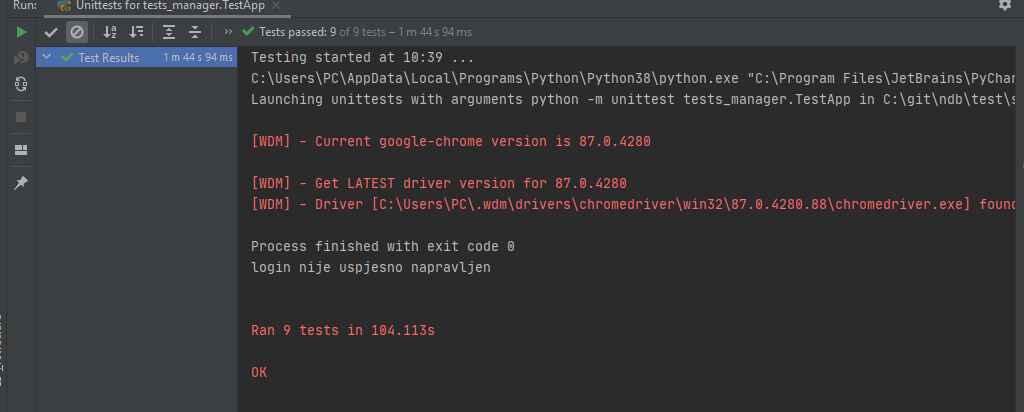
\includegraphics[scale=0.6]{slike/test_sistem_rezultat.png} %veličina slike u odnosu na originalnu datoteku i pozicija slike
				\centering
				\caption{Prikaz rezultata nakon provedenog ispitivanja}
				\label{fig:test - sistemski - rezultat}
			\end{figure}					
	
			%unos slike
			\begin{figure}[H]
				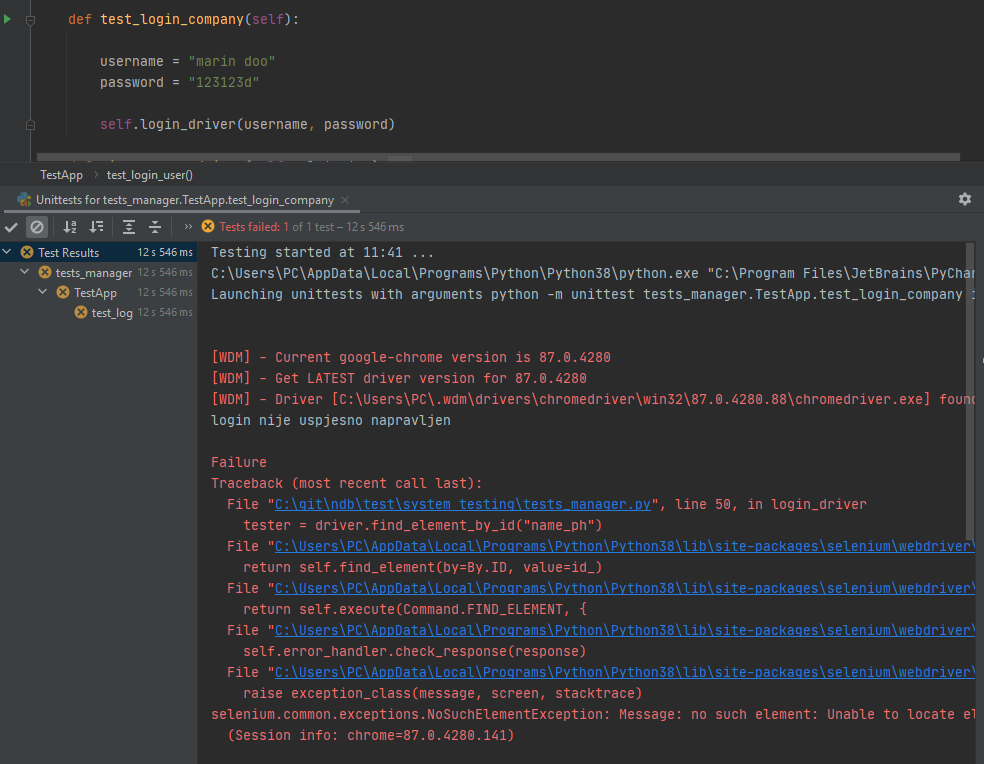
\includegraphics[scale=0.6]{slike/test_sistem_failedTest.png} %veličina slike u odnosu na originalnu datoteku i pozicija slike
				\centering
				\caption{Prikaz primjera rezultata u slučaju da očekujemo rezultat drugačiji od dobivenog (provedeni test je prikazani)}
				\label{fig:test - sistemski - neuspješno provedeni test}
			\end{figure}					
			
			\eject 
		
		
		\section{Dijagram razmještaja}
			 
			 Dijagram razmještaja je strukturni UML dijagram koji opisuje topologiju sustava i prikazuje odnos između sklopovskih i programskih dijelova. Poslužiteljsku stranu predstavlja \textit{cloud} platforma Heroku. Na Heroku se nalaze web poslužitelj i poslužitelj baze podataka, a pristupa kartama omogućen je preko \textit{Google API} servisa. Na klijentskoj strani koristi se web preglednik kojim se pristupa web aplikaciji. Komunikacija između korisnika i oblaka odvija se putem HTTPS veze.
			
			\begin{figure}[H]
				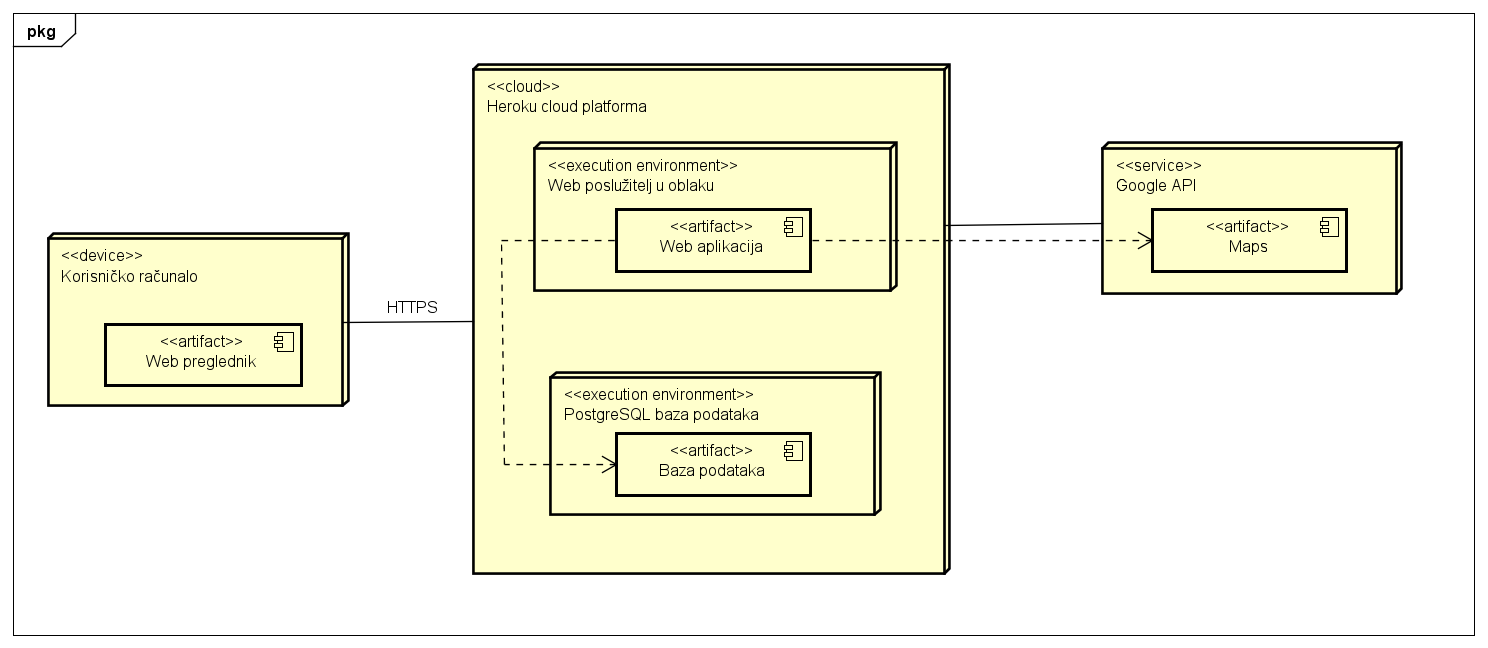
\includegraphics[scale=0.45]{dijagrami/dijagram_razmjestaja.png} %veličina slike u odnosu na originalnu datoteku i pozicija slike
				\centering
				\caption{Dijagram razmještaja}
				\label{fig:promjene}
			\end{figure}
			
			\eject 
		
		\section{Upute za puštanje u pogon}
		
		
			Pokretanje Stranice preko Heroku-a:
			\begin{itemize}
				\item 	\textit{Prvo se treba ulogirati na Heroku}
				\item 	\textit{Nakon logina treba se povezati postojeći git repozitorij sa Heroku-om pozivanjem
					“heroku git:remote -a imestranice”}
				\item 	\textit{Nakon povezivanja repozitorij se može pushati sa “git push heroku master” u slučaju da se pusha sa Master brancha ili “git push heroku imebrancha:master”}		
				
				\item 	\textit{Nakon što se repozitorij pusha na Heroku, potrebno je napraviti bazu podataka.}	
				
				\item 	\textit{Na Resources stranici Heroku-a kao add-on se doda Heroku Postgres te se iz dane baze trebaju uzeti podatci za spajanje}
				
				\item 	\textit{Nakon toga se u konzoli pozove “heroku run bash” kojim se otvori bash te se u bashu pokrene seed.js kako bi se napravila baza podataka}
	
				\item 	\textit{Kada je to napravljeno, web stranica se može pokrenuti}
			\end{itemize}
		
		
			

		
					%unos slike
		\begin{figure}[H]
			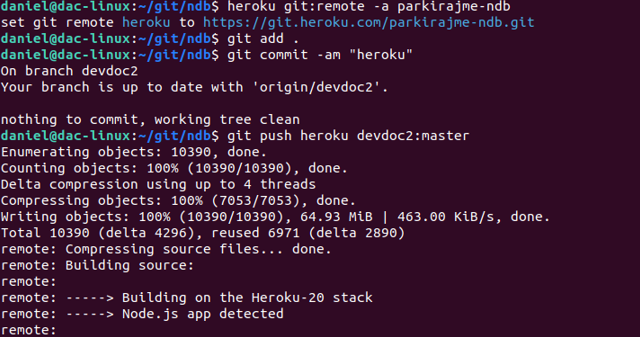
\includegraphics[scale=0.8]{slike/heroku_s1.png} %veličina slike u odnosu na originalnu datoteku i pozicija slike
			\centering
			\caption{Upravljanje Heroku-om}
			\label{fig:Upravljanje Heroku-om 1}
		\end{figure}
	
				%unos slike
	\begin{figure}[H]
		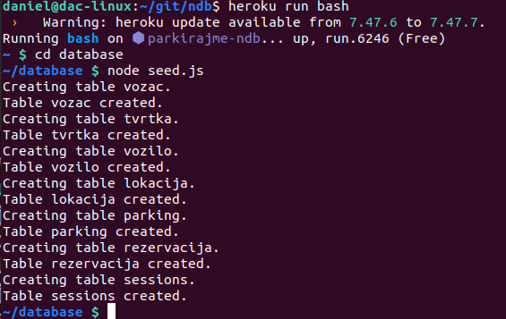
\includegraphics[scale=0.8]{slike/heroku_s2.png} %veličina slike u odnosu na originalnu datoteku i pozicija slike
		\centering
		\caption{Kreiranje baze podataka}
		\label{fig:Upravljanje Heroku-om 2}
	\end{figure}
			
			\eject 